\section{Database Planning}\label{sec:database_planning}

When we were assigned this project, the database system did not fully support saving sequences of pictograms. The database was built to save only pictograms to profile, and you had to create code to interpret which pictograms were part of what sequences. This was not ideal and required a lot of work to use. Additionally, it required users to search through all pictograms every time you had to open a sequence. We gathered with all of the groups who had interest in saving sequences in the database. The groups were the following Livshistorier, PiktoOplæser and the iOS group.
When collaborating to find a joint database system for groups with different needs, we needed a set of requirements from each groups. We arranged a meeting and discussed the different requirements and created design conventions for each user story, thereafter deciding what the minimal common we could reach was. 

Each group were to present an ER-model or idea for a database that entailed all of the features that were needed for the minimal database design. The draft we came up with are portrayed in \ref{fig:DBdescription}:
\begin{figure}
\centering
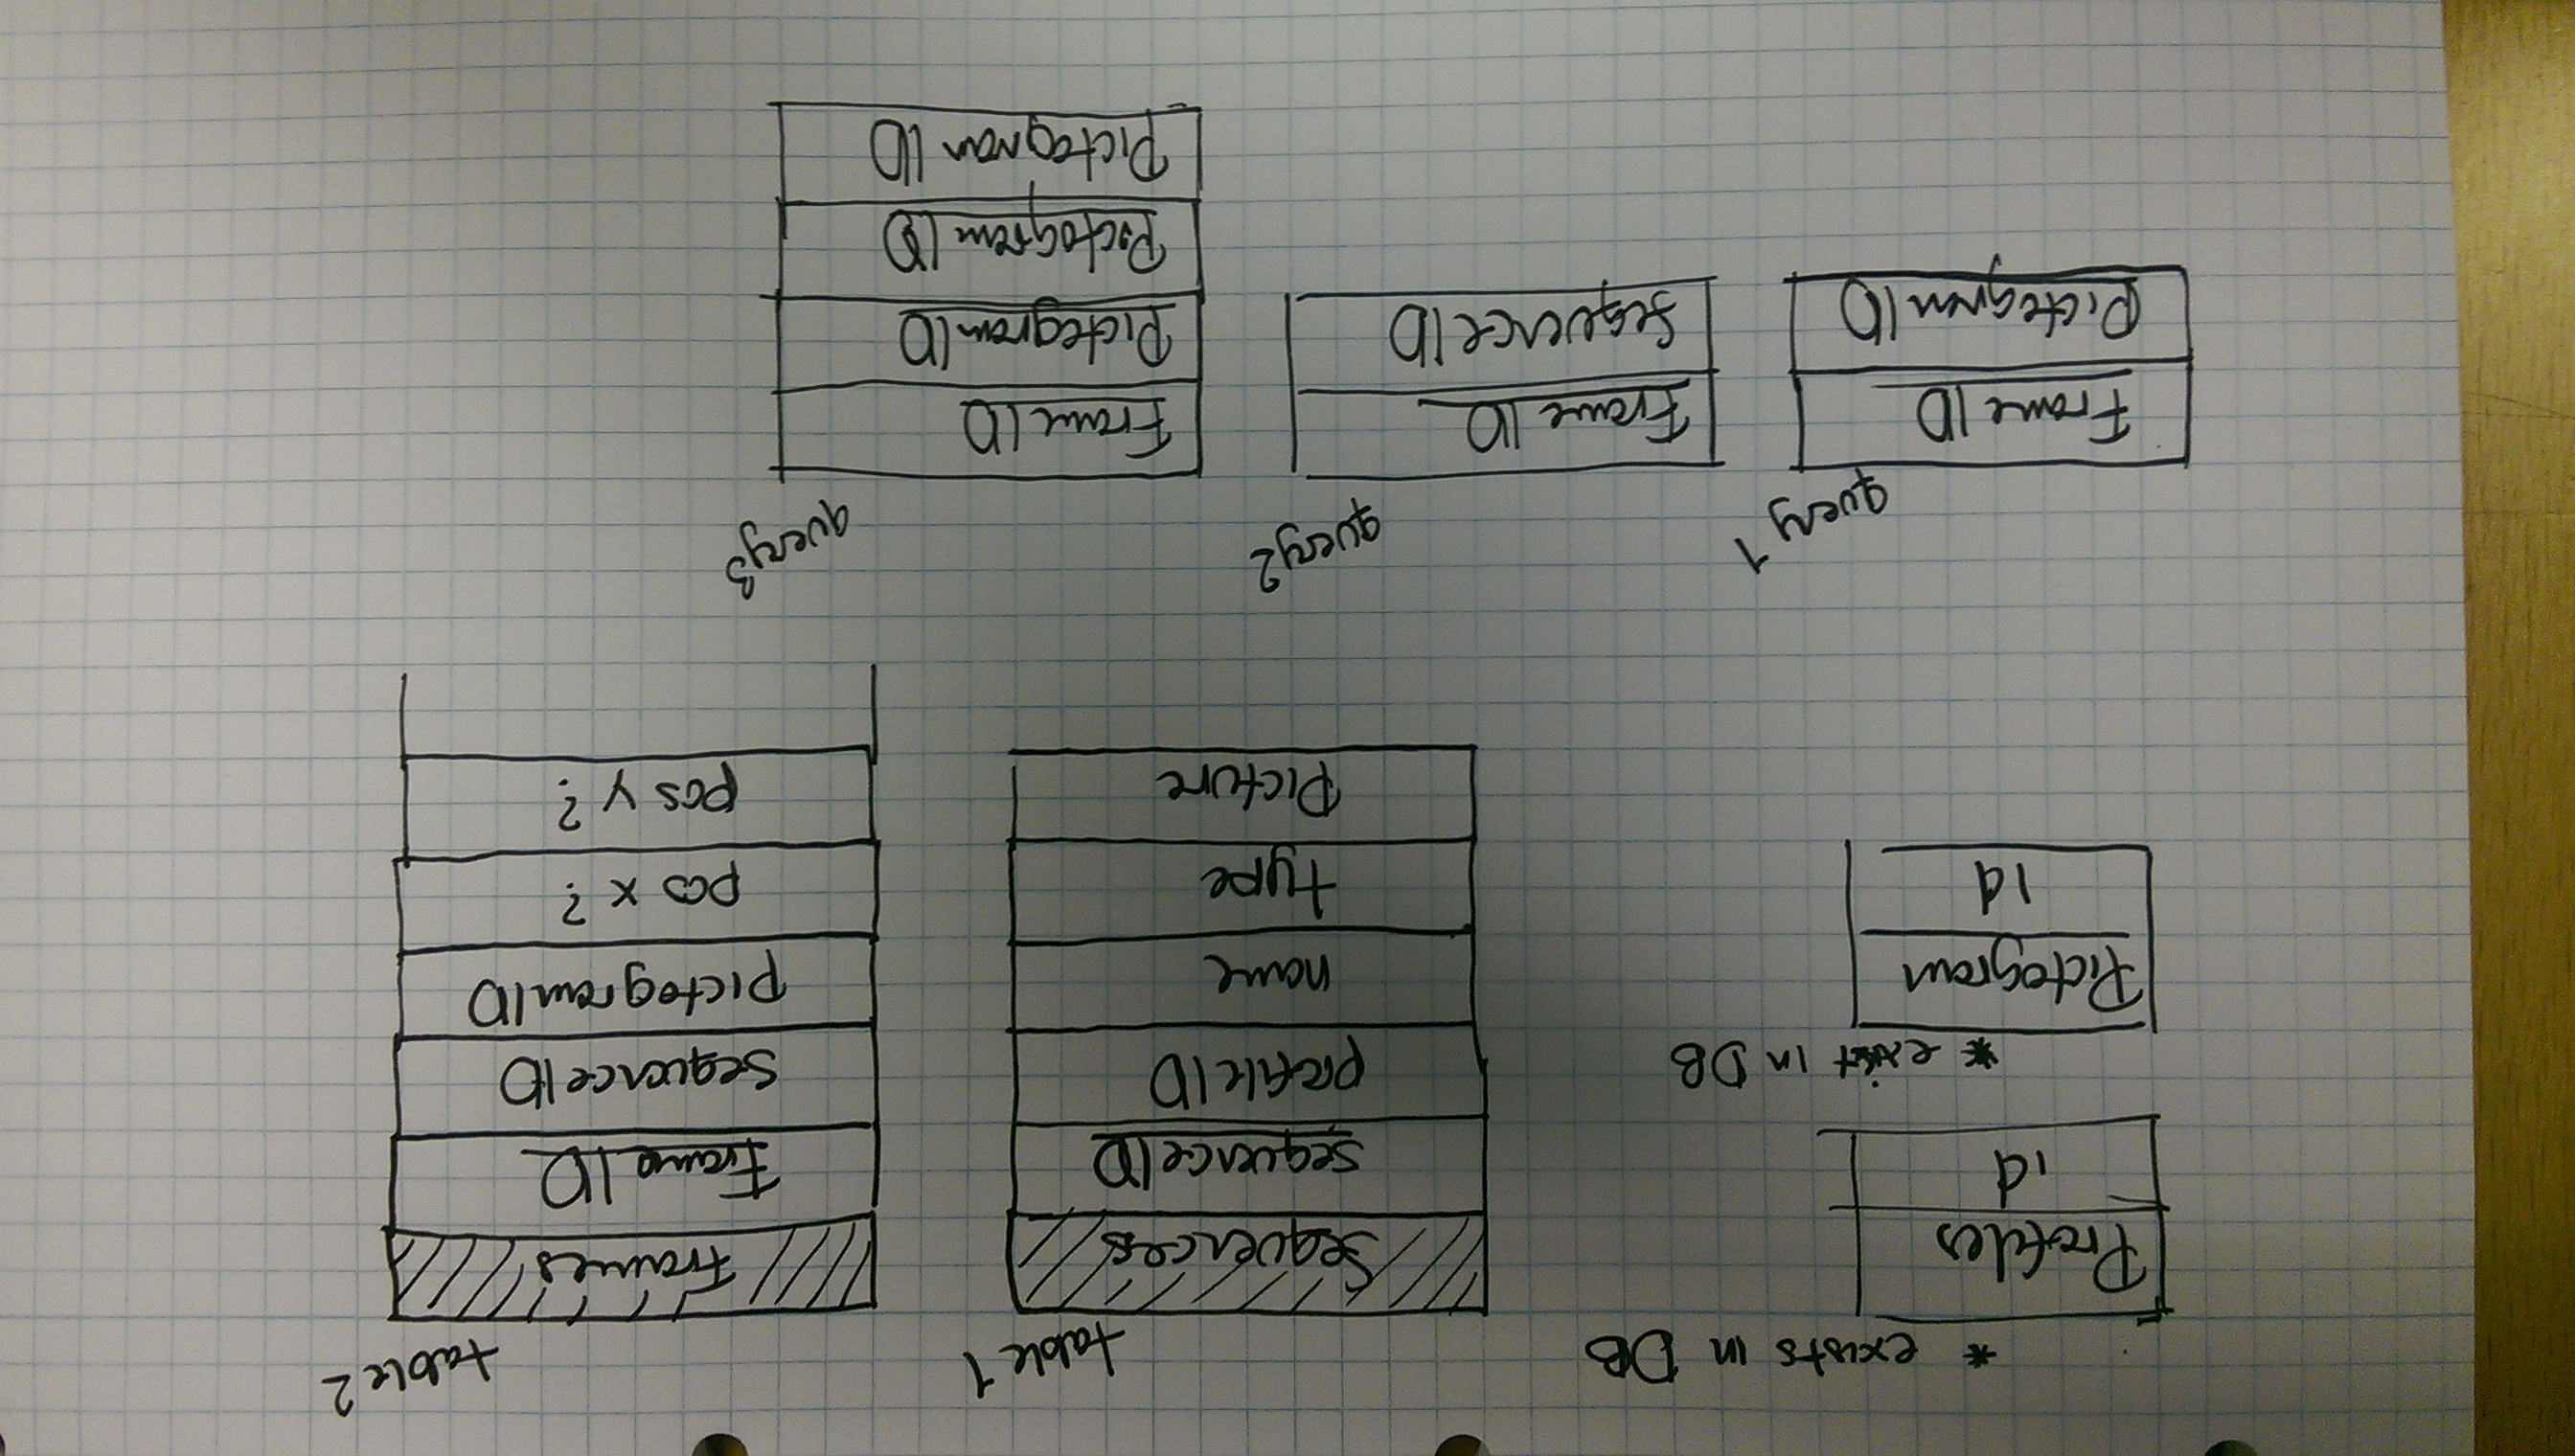
\includegraphics[width=0.7\linewidth]{Pics/ourDBdescription}
\caption{Our idea of a potential database for sequences}
\label{fig:DBdescription}
\end{figure}

As profiles and pictograms already exists in the database, these tables are not further described. We add a new sequence table that contains all of the information needed to describe a sequence from all of the groups, there is nothing really questionable here. The second table, Frames, is where the most of the magic happen. The way the pictograms/nested sequences/choices are saved in the database are that they are saved to each frame. A frame can store one or more pictograms, or a nested sequenceId. This way when you are fetching a sequence from the database, you search the list of frames for frames matching the sequenceId and setting them up according to posX.\newline
\newline
The draft we submitted was quickly decided as a good baseline, but Livshistorier refined it by removing the choice table, as this was possible to create through the pictogram table. We agreed that Livshistorier would collaborate with OasisLib on converting the draft to an official ER-diagram. 